%%%%%%%%%%%%%%%%%%%%%%%%%%%%%%%%%%%%%%%%%%%%%%%%%
\chapter{ΜΕΘΟΔΟΙ ΠΡΟΒΛΕΨΗΣ}
%%%%%%%%%%%%%%%%%%%%%%%%%%%%%%%%%%%%%%%%%%%%%%%%%
\section{ ΚΡΙΤΗΡΙΑ ΑΞΙΟΛΟΓΗΣΗΣ ΤΩΝ ΜΕΘΟΔΩΝ ΠΡΟΒΛΕΨΗΣ}
Η ανάλυση χρονοσειρών (time series analysis) ασχολείται αποκλειστικά με τη
διερεύνηση της διαχρονικής συμπεριφοράς των τιμών μιας μεταβλητής, οι
παρατηρήσεις της οποίας προέρχονται από χρονοσειρά. Η πρόβλεψη των
μελλοντικών τιμών της μεταβλητής σύμφωνα με την ανάλυση χρονοσειρών μπορεί
να προέλθει απο διάφορες κατηγορίες μεθόδων προβλέψης, όπως η μέθοδος Εξομάλυνσης και η Διάσπαση των χρονοσειρών, με τις οποίες θα ασχοληθούμε στην παρούσα εργασία.\\
Για την επιλογή της κατάλληλης μεθόδου χρησιμοποιούνται τα κριτήρια
αξιολόγησης των μεθόδων προβλέψεων. Τα κριτήρια αυτά βασίζονται στις τιμές των
αποκλίσεων των προβλεπόμενων τιμών από τις αντίστοιχες πραγματικές τιμές της
χρονοσειράς.\\
Για μία μεταβλητή Y, η απόκλιση της προβλεπόμενης τιμής της $ \widehat{Y}_t $  από την
αντίστοιχη πραγματική τιμή της $Y_t$ για την περίοδο t, όπου $t=1,2,3,\ldots,n , \:$ ονομάζεται
σφάλμα της πρόβλεψης (forecast error), συμβολίζεται με $e_t$ και ορίζεται ως:
$\: e_t = Y_t - \widehat{Y}_t$\\
Η παραπάνω σχέση εκφράζει για κάθε περίοδο t τη διαφορά μεταξύ της πραγματικής
τιμής $Y_t$ και της αντίστοιχης προβλεπόμενης τιμής $ \widehat{Y}_t $ που προήλθε από τη μέθοδο
πρόβλεψης που χρησιμοποιήθηκε.\\
Επομένως, για να προσδιορίσουμε την αξιοπιστία μιας συγκεκριμένης μεθόδου
πρόβλεψης, θα πρέπει να μελετήσουμε τη διαχρονική συμπεριφορά των τιμών των
σφαλμάτων της πρόβλεψης. Αυτό γίνεται με την εφαρμογή διάφορων κριτηρίων,
σύμφωνα με τα οποία αξιολογούμε τη χρησιμοποιούμενη μέθοδο πρόβλεψης. Κάθε
ένα από τα κριτήρια αυτά ορίζεται από μία συγκεκριμένη συναρτησιακή σχέση των
σφαλμάτων της πρόβλεψης και μπορεί να χρησιμοποιηθεί όχι μόνο για την
αξιολόγηση μιας μεθόδου πρόβλεψης αλλά και για την επιλογή της “ καλύτερης ”
μεταξύ δύο ή περισσοτέρων εναλλακτικών μεθόδων προβλέψεων. Τα κριτήρια αυτά
είναι:\\
\begin{itemize}
\item \textbf{Μέση απόλυτη απόκλιση MAD} (Mean Absolute Deviation)\\
Η μέση απόλυτη απόκλιση ορίζεται ως το άθροισμα των απόλυτων τιμών του
σφάλματος της πρόβλεψης διαιρούμενο με τον αριθμό των περιόδων n, στις οποίες
έγιναν προβλέψεις, δηλαδή:\\
$$ MAD= \frac{1}{n} \sum_{t=1}^n \vert Y_t-\widehat{Y}_t \vert =\frac{1}{n} \sum_{t=1}^n \vert e_t \vert $$
Το MAD εκφράζει τη μέση τιμή των απολύτων αποκλίσεων των προβλεπόμενων
τιμών της χρονοσειράς από τις αντίστοιχες πραγματικές και έχει τα ακόλουθα
χαρακτηριστικά. Πρώτον, η μονάδα μέτρησης του είναι η ίδια με εκείνη των τιμών
της χρονοσειράς και έτσι είναι εύκολη η ερμηνεία του. Δεύτερον, στον υπολογισμό
του λαμβάνονται υπ’ όψιν μόνο οι απόλυτες τιμές των σφαλμάτων και όχι οι
πραγματικές τιμές τους. Αυτό σημαίνει ότι το MAD είναι ανεξάρτητο από θετικές ή αρνητικές τιμές του σφάλματος, δηλαδή είναι ανεξάρτητο από το αν οι τιμές των
προβλέψεων είναι μικρότερες ή μεγαλύτερες των
πραγματικών τιμών.Και τέλος, το MAD βασίζεται στην υπόθεση ότι η αξιοπιστία του
σφάλματος ή το κόστος που δημιουργείται από το σφάλμα της πρόβλεψης, σχετίζεται
γραμμικά με το μέγεθος του σφάλματος.

\item \textbf{ Μέσο σφάλμα τετραγώνου MSE} (Mean Squared Error)\\
Το μέσο σφάλμα τετραγώνου ορίζεται ως το άθροισμα των τετραγώνων των
σφαλμάτων διαιρούμενο με τον αριθμό των χρονικών περιόδων n, στις οποίες έγιναν οι
προβλέψεις, δηλαδή:\\
$$ MSE= \frac{1}{n} \sum_{t=1}^n \left( Y_t-\widehat{Y}_t \right)^2 =\frac{1}{n} \sum_{t=1}^n  e_t^2 $$
Το MSE είναι η μέση τιμή των τετραγώνων των αποκλίσεων των προβλεπόμενων
τιμών της χρονοσειράς από τις αντίστοιχες πραγματικές. Η μονάδα μέτρησης του
MSE είναι εκφρασμένη στη μονάδα μέτρησης των τιμών των παρατηρήσεων
υψωμένη στο τετράγωνο.\\
Η ύπαρξη προβλέψεων που απέχουν πολύ από τις αντίστοιχες πραγματικές τιμές
γίνεται πολύ περισσότερο αισθητή με το κριτήριο MSE από ότι με το κριτήριο MAD,
επειδή οι τιμές των σφαλμάτων της πρόβλεψης υψώνονται στο τετράγωνο. Συνεπώς
το κριτήριο MSE είναι στατιστικά περισσότερο αξιόπιστο από το κριτήριο MAD και
χρησιμοποιείται συχνότερα για την επιλογή της ‘κατάλληλης’ μεθόδου πρόβλεψης.

\item \textbf{Ρίζα μέσου
σφάλματος τετραγώνου RMSE} (Root Mean Squared Error)\\
H τετραγωνική ρίζα μέσου
σφάλματος τετραγώνου είναι η
θετική τιμή της τετραγωνικής του ρίζας, δηλαδή είναι:\\
$$ RMSE=\sqrt{MSE}=\sqrt{\frac{1}{n}\sum_{t=1}^n e_t^2} $$
Το RMSE εκφράζεται στην ίδια μονάδα μέτρησης με εκείνη των τιμών της
χρονοσειράς.\\


\item \textbf{Μέσο απόλυτο ποσοστιαίο σφάλμα MAPE} (Mean Absolute Percentage
Error)\\
Το μέσο απόλυτο ποσοστιαίο σφάλμα εξετάζει τη συμπεριφορά της απόλυτης
τιμής του σφάλματος της πρόβλεψης σε σχέση με την πραγματική τιμή της
χρονοσειράς. Το MAPE ορίζεται ως το άθροισμα των απόλυτων τιμών των
σφαλμάτων της πρόβλεψης προς τις αντίστοιχες πραγματικές τιμές της χρονοσειράς
διαιρούμενο με τον αριθμό των χρονικών περιόδων n, στις οποίες έγιναν προβλέψεις,
δηλαδή:\\
$$MAPE= \frac{1}{n} \sum_{t=1}^n \frac{\vert Y_t-\widehat{Y}_t \vert}{Y_t}=\frac{1}{n}\sum_{t=1}^n \frac{\vert e_t \vert}{Y_t} $$
Το κριτήριο αυτό είναι απαλλαγμένο από μονάδες μέτρησης και το
χρησιμοποιούμε για να συγκρίνουμε την ακρίβεια μιας ή περισσοτέρων μεθόδων
προβλέψεων και για περισσότερες από μια χρονοσειρές.

\item \textbf{Μέσο ποσοστιαίο σφάλμα MPE} (Mean Percentage Error)\\
Το μέσο ποσοστιαίο σφάλμα το χρησιμοποιούμε όταν ενδιαφερόμαστε να
προσδιορίσουμε αν η μέθοδος πρόβλεψης είναι μεροληπτική, δηλαδή αν οι
προβλεπόμενες τιμές είναι συστηματικά μεγαλύτερες ή μικρότερες από τις
αντίστοιχες πραγματικές.\\
$$ MPE= \frac{1}{n} \sum_{t=1}^n \frac{Y_t-\widehat{Y}_t}{Y_t} =\frac{1}{n} \sum_{t=1}^n \frac{e_t}{Y_t}$$
Χωρίς αμφιβολία, όσο πιο κοντά στο μηδέν είναι η τιμή του MPE, τόσο πιο
αμερόληπτη και καλή είναι η μέθοδος πρόβλεψης που χρησιμοποιήθηκε. Αντιθέτως,
μεγάλες απόλυτες τιμές του MPE φανερώνουν μεγάλη μεροληψία της μεθόδου.


\end{itemize}


%%%%%%%%%%%%%%%%%%%%%%%%%%%%%%%%%%%%%%%%%%%%%%%
\section{ΜΕΘΟΔΟΙ ΕΞΟΜΑΛΥΝΣΗΣ}
%%%%%%%%%%%%%%%%%%%%%%%%%%%%%%%%%%%%%%%%%%%%%%%

Οι μέθοδοι εξομάλυνσης (smoothing methods) είναι τεχνικές με τις οποίες
προσδιορίζονται οι μελλοντικές τιμές μιας μεταβλητής με βάση τον τρόπο εφαρμογής
τους. Οι τεχνικές αυτές ονομάζονται μέθοδοι εξομάλυνσης, διότι η δημιουργία των
προβλέψεων προέρχεται από την εξομάλυνση της διαχρονικής εξέλιξης των τιμών της
μεταβλητής, ώστε να αναγνωριστεί καλύτερα ο τρόπος συμπεριφοράς της. Ορισμένες
από τις μεθόδους εξομάλυνσης μπορούν να εφαρμοστούν και σε περιπτώσεις μικρού
αριθμού παρατηρήσεων της μεταβλητής. Οι μέθοδοι εξομάλυνσης που θα
περιγράψουμε είναι:\\
\begin{itemize}
\item Η μέθοδος του απλού κινητού μέσου
\item Η μέθοδος της απλής εκθετικής εξομάλυνσης
\item Η μέθοδος του διπλού κινητού μέσου
\item Η μέθοδος Brown
\item Η μέθοδος Holt
\item Η μέθοδος Winters
\end{itemize}

Εάν μία χρονοσειρά είναι στάσιμη η κατάλληλη μέθοδος πρόβλεψης μελλοντικών
τιμών είναι η μέθοδος των κινητών μέσων όρων. Σε μερικές χρονοσειρές όμως οι
πρόσφατες παρατηρήσεις μπορεί να περιέχουν περισσότερες πληροφορίες από τις
παλαιότερες και αυτό είναι πολύ σημαντικό για τις μελλοντικές προβλέψεις. Σε αυτήν
την περίπτωση χρησιμοποιούμε την απλή εκθετική εξομάλυνση. Εάν η χρονοσειρά
εμφανίζει κάποιο πρότυπο τάσης τότε χρησιμοποιούμε την μέθοδο της διπλής
εκθετικής εξομάλυνσης, την μέθοδο Brown ή την μέθοδο Holt ενώ εάν η χρονοσειρά
εμφανίζει εποχικότητα τότε χρησιμοποιούμε την μέθοδο Winters.

%%%%%%%%%%%%%%%%%%%%%%%%%%%%%%%%%%%%%%%%%%%%%%%
\subsection{ΑΠΛΟΣ ΚΙΝΗΤΟΣ ΜΕΣΟΣ}
%%%%%%%%%%%%%%%%%%%%%%%%%%%%%%%%%%%%%%%%%%%%%%%
Η μέθοδος του απλού κινητού μέσου m-περιόδων (simple moving average) είναι
μία πολύ απλή μέθοδος προβλέψεων που χρησιμοποιεί ως πρόβλεψη την τιμή του
αριθμητικού μέσου όρου των m πλέον πρόσφατων παρατηρήσεων της χρονοσειράς.
Αυτό συμβαίνει διότι οι πλέον πρόσφατες παρατηρήσεις της χρονοσειράς θεωρούνται
περισσότερο αντιπροσωπευτικές για τη δημιουργία προβλέψεων από ότι οι πιο
απομακρυσμένες στο παρελθόν. Ο μέσος όρος αυτός ονομάζεται κινητός, επειδή η
τιμή του δεν είναι σταθερή, αλλά αναπροσαρμόζεται κάθε φορά που μια νέα
παρατήρηση της χρονοσειράς γίνεται διαθέσιμη.\\
Οι προβλέψεις μιας χρονοσειράς $Y_t$ , για $t=1,2,\ldots,n \:\:$, δημιουργούνται με τη μέθοδο
του απλού κινητού μέσου ως εξής:\\
$$ \widehat{Y}_{t+1}=\frac{1}{m}\sum_{j=1}^m Y_{t-j+1}=\frac{1}{m} \left(Y_t +Y_{t-1}+\ldots+Y_{t-m+1}\right) $$
όπου $\widehat{Y}_{t+1} $ είναι η πρόβλεψη για την περίοδο $(t+1)$ \\
και $m $ είναι ο αριθμός των περιόδων που
χρησιμοποιούνται για τον υπολογισμό της τιμής του μέσου όρου.
Επίσης, για m=1 η πρόβλεψη της επόμενης περιόδου είναι ίση με την πραγματική τιμή της προηγούμενης περιόδου, δηλαδή ισχύει η σχέση:
$\: \widehat{Y}_{t+1}=Y_t $ \\

Απαραίτητη προϋπόθεση για την εφαρμογή του ανωτέρω τύπου είναι ο
προσδιορισμός του m. Η τιμή του m δύναται να είναι γνωστή, οπότε χωρίς
καμία δυσκολία μπορούμε να δημιουργήσουμε την πρόβλεψη της περιόδου
(t+1), δύναται όμως να είναι και άγνωστη. Στην περίπτωση που η τιμή του m
δεν είναι προκαθορισμένη (η περίπτωση αυτή αποτελεί το πλέον σύνηθες
φαινόμενο) τότε ο ερευνητής καλείται με βάση την κρίση του, την εμπειρία του και τα δεδομένα των παρατηρήσεων της χρονοσειράς να προσδιορίσει την
τιμή του m. Συνήθως, για να προσδιοριστεί η τιμή του m για μια συγκεκριμένη χρονοσειρά υπολογίζεται ο απλός κινητός μέσος για διάφορες τιμές του m και
επιλέγεται εκείνη η τιμή που ελαχιστοποιεί την τιμή ενός κριτηρίου, από εκείνα που υπάρχουν, για την αξιολόγηση των μεθόδων προβλέψεων (συνήθως του
MSE ή του RMSE).\\

Με τη μέθοδο του απλού κινητού μέσου μπορούμε να εξομαλύνουμε τις τιμές
της χρονοσειράς. Αναλυτικότερα, εφαρμόζοντας τον παραπάνω μαθηματικό τύπο  στις παρατηρήσεις της χρονοσειράς, εξομαλύνουμε
τις τελευταίες (n – m) παρατηρήσεις της χρονοσειράς. Οι τιμές που
προκύπτουν χρησιμοποιούνται ως προβλέψεις των αντίστοιχων περιόδων και
εν συνεχεία, βάσει αυτών, προσδιορίζουμε τις τιμές των σφαλμάτων της
πρόβλεψης.\\

%%%%%%%%%%%%%%%%%%%%%%%%%%%%%%%%%%%%%%%%%%%%%
\subsection{ΑΠΛΗ ΕΚΘΕΤΙΚΗ ΕΞΟΜΑΛΥΝΣΗ}
%%%%%%%%%%%%%%%%%%%%%%%%%%%%%%%%%%%%%%%%%%%%%
Ένα μειονέκτημα της μεθόδου του απλού κινητού μέσου m-περιόδων είναι ότι για
τον υπολογισμό των προβλέψεων δίνει ίση βαρύτητα σε κάθε παρατήρηση,
ανεξάρτητα από το πόσο κοντά ή μακριά βρίσκεται σε σχέση με την προβλεπόμενη περίοδο. Το μειονέκτημα αυτό μπορεί να εξαλειφθεί με τη μέθοδο της απλής εκθετικής εξομάλυνσης (simple exponential smoothing), σύμφωνα με την οποία οι προβλέψεις δημιουργούνται με βάση κάποιο σταθμικό μέσο όρο, έτσι ώστε να δίνεται
διαφορετική βαρύτητα σε κάθε παρατήρηση. Πιο συγκεκριμένα, με τη μέθοδο αυτή
δίνεται πολύ μεγαλύτερη βαρύτητα στις πιο πρόσφατες παρατηρήσεις, από αυτή που
δίνεται στις πιο απομακρύσμενες.\\
Για να κατανοήσουμε το μηχανισμό λειτουργίας της μεθόδου ας θεωρήσουμε ότι
οι προβλέψεις της χρονοσειράς δημιουργούνται ως εξής:\\
\begin{equation}
\label{ekthetikh}
 \widehat{Y}_{t + 1} = aY_t + a \left( 1 − a \right) Y_{t − 1} + a \left( 1 − a \right)^2 Y_{t − 2} + \dots 
\end{equation}
που η παράμετρος α ονομάζεται σταθερά εξομάλυνσης (smoothing constant) και
λαμβάνει τιμές μεταξύ 0 και 1 δηλαδή: $ \: 0\leq a\leq 1$\\
Έτσι, σύμφωνα με την παραπάνω σχέση η πρόβλεψη $\widehat{Y}_{t+1} $ προκύπτει ως ένας
σταθμικός μέσος όρος των παρατηρήσεων της χρονοσειράς, αφού το άθροισμα των
συντελεστών της σχέσης $\left(\ref{ekthetikh}\right) $ είναι ίσο με τη μονάδα. Όσο πιο μεγάλη είναι η τιμή της
παραμέτρου α, τόσο μεγαλύτερη βαρύτητα δίνεται στις πιο πρόσφατες παρατηρήσεις
και πολύ μικρή εως μηδαμινή βαρύτητα στις πιο απομακρυσμένες.\\
Η παραπάνω σχέση μπορεί να γραφεί και με τη μορφή:\\
\begin{equation}
\widehat{Y}_{t + 1} = aY_t + \left( 1 − a \right) \widehat{Y}_t 
\end{equation}
Η σχέση αυτή είναι η μαθηματική έκφραση της μεθόδου της απλής εκθετικής
εξομάλυνσης και ορίζεται για $\:t=2,3,\ldots,n\:$ με αρχική συνθήκη $\widehat{Y}_2 = Y_1$ .\\\\
%Η τιμή της παραμέτρου α καθορίζεται από τον ερευνητή. Ωστόσο, πιο
%αντικειμενικό είναι η “άριστη” τιμή του α να προσδιορίζεται από τα δεδομένα της
%χρονοσειράς. Ειδικότερα, εφαρμόζοντας τη μέθοδο της απλής εκθετικής εξομάλυνσης
%στις παρατηρήσεις της χρονοσειράς, για τιμές του α από το μηδέν μέχρι τη μονάδα
%επιλέγουμε εκείνη την τιμή του α που ελαχιστοποιεί την τιμή του κριτηρίου MSE ή
%κάποιου άλλου κριτηρίου.
Είναι προφανές ότι η πρόβλεψη $ \widehat{Y}_{t+1}$ της περριόδου $\left( t+1 \right)$ είναι ένας σταθμικός μέσος όρος της πραγματικής τιμής $ Y_t$ και της προβλεπόμενης τιμής $ \widehat{Y}_t$ 
της περιόδου $t$ με συντελεστές βαύτητας $a$ και $\left(1-a \right)$ αντίστοιχα. Πρακτικά, αυτό σημαίνει ότι εάν η τιμή της σταθεράς εξομάλυνσης  είναι $ a=0,3 $, τότε η πρόβλεψη της επόμενης περιόδου προσδιορίζεται κατά $30 \%$ απ' την πραγματική τιμή και κατά $70 \%$ απ' την προβλεπόμενη τιμή της τρέχουσας περιόδου. Να σημειωθεί πως όταν η τιμή της σταθεράς εξομάλυνσης λαμβάνει τις ακραίες τιμές ένα και μηδέν τότε: \\
\begin{itemize}
\item για $a=1$ η πρόβλεψη της επόμενης περιόδου $\left(t+1\right)$ είναι η πραγματική τιμή της τρέχουσας περιόδου t 
\item για $a=0$ η πρόβλεψη της επόμενης περιόδου $\left(t+1\right)$ είναι ίση με την
πρόβλεψη της τρέχουσας περιόδου t.
\end{itemize}

Παρατηρούμε ότι όσο πιο μικρές είναι οι τιμές της σταθεράς $a$ τόσο
περισσότερο εξομαλύνονται οι παρατηρήσεις της χρονοσειράς και όσο πιο
μεγάλες είναι οι τιμές της σταθεράς $a$ τόσο πιο γρήγορα αντιδρά η εν λόγω
μέθοδος στις πραγματικές μεταβολές των παρατηρήσεων της χρονοσειράς.
Συνεπώς τίθεται ένα ερώτημα : Μεγαλύτερη εξομάλυνση των παρατηρήσεων
της χρονοσειράς και άρα μικρή τιμή για το $a$ ή μεγαλύτερη ανταπόκριση στις
πραγματικές μεταβολές των παρατηρήσεων και άρα μεγάλη τιμή για το $a$ ; Η
απάντηση στο ερώτημα αυτό δεν είναι καθόλου εύκολη. Θα λέγαμε ότι
σπουδαίο ρόλο διαδραματίζει η κρίση του ερευνητή και η τυχόν προηγούμενη
εμπειρία που έχει για τη συγκεκριμένη χρονολογική σειρά. Βέβαια, το πιο
σωστό είναι η «άριστη» τιμή για το $a$ να προσδιορίζεται από τα δεδομένα της
χρονοσειράς. Συγκεκριμένα από τις τιμές του $a$, $0 \leq a \leq 1$, επιλέγουμε εκείνη
που ελαχιστοποιεί την τιμή του κριτηρίου MSE ή κάποιου άλλου κριτηρίου.\\\\
Η μαθηματική σχέση που εκφράζει τη μέθοδο της απλής εκθετικής
εξομάλυνσης μπορεί να λάβει και την ακόλουθη μορφή :\\
\begin{equation}
\label{ekth}
\widehat{Y}_{t+1}=\widehat{Y}_t + a\left( Y_t - \widehat{Y}_t \right) = \widehat{Y}_t + a e_t 
\end{equation}
Η σχέση $\left(\ref{ekth}\right) $ μας δείχνει ότι η πρόβλεψη της περιόδου (t+1) είναι ίση με την πρόβλεψη της περιόδου t συν το σφάλμα της πρόβλεψης $e_t$ ,
πολλαπλασιασμένο με την τιμή της σταθεράς εξομάλυνσης $a$. Κατά συνέπεια
όσο μεγαλύτερη είναι η τιμή του $a$, τόσο πιο μεγάλη βαρύτητα δίνεται στο
σφάλμα της πρόβλεψης.
%%%%%%%%%%%%%%%%%%%%%%%%%%%%%%%%%%%%%%%%%%%
\subsection{ΔΙΠΛΟΣ ΚΙΝΗΤΟΣ ΜΕΣΟΣ}
%%%%%%%%%%%%%%%%%%%%%%%%%%%%%%%%%%%%%%%%%%%

Όταν οι παρατηρήσεις της χρονοσειράς που εξετάζουμε παρουσιάζουν μια ανοδική ή πτωτική εξελικτική πορεία που εκφράζεται από κάποια γραμμική
τάση, τότε μπορούμε να χρησιμοποιήσουμε τη μέθοδο του διπλού κινητού μέσου (double moving average) για την πρόβλεψη των τιμών της χρονοσειράς. Για τη διαμόρφωση των προβλέψεων με τη μέθοδο αυτή
υπολογίζεται ένας δεύτερος κινητός μέσος από τον απλό κινητό μέσο, ενώ στη συνέχεια λαμβάνεται υπ' ́όψιν και η γραμμική τάση των παρατηρήσεων της
χρονοσειράς . Για το λόγο αυτό η μέθοδος ονομάζεται πολύ συχνά και μέθοδος του
γραμμικού κινητού μέσου (linear moving average).\\\\
Η εφαρμογή της μεθόδου του διπλού κινητού μέσου βασίζεται στην ακόλουθη
διαδικασία:\\
\begin{enumerate}
\item Αρχικά, υπολογίζουμε τον απλό κινητό μέσο m-περιόδων,$\: M_t$ , ως εξής:\\
$$ M_{t+1}=\frac{1}{m} \sum_{j=1}^m Y_{t-j+1} $$
\item Στη συνέχεια, υπολογίζουμε τον διπλό κινητό μέσο m-περιόδων, $M^{'}_t, $:\\
$$ M^{'}_{t+1}= \frac{1}{m} \sum_{j=1}^m M_{t-j+1} $$
\item Ύστερα, βρίσκουμε τη διαφορά $a_t$:\\
$$a_t=2M_t-M^{'}_t $$
\item Βρίσκουμε τον παράγοντα προσαρμογής για την τάση, $b_t$ :\\
$$ b_t=\frac{2}{m-1} \left(M_t -M^{'}_t \right)$$ 
\item Και τέλος, υπολογίζουμε την πρόβλεψη $\widehat{Y}_{t + h}$ για την h μελλοντική περίοδο ως εξής:\\
$$ \widehat{Y}_{t+h}=a_t+hb_t $$
όπου h είναι ένας ακέραιος θετικός αριθμός.\\
\end{enumerate}

Η μέθοδος αυτή, σε αντίθεση με τη μέθοδο του απλού κινητού  μέσου όρου που
παρουσιάσαμε, μπορεί για $h>1$ να χρησιμοποιηθεί για τη διαμόρφωση προβλέψεων για
περισσότερες από μία μελλοντικές περιόδους, ενώ για $h=1$ δίνει την πρόβλεψη για
την επόμενη περίοδο. Βέβαια, η χρήση της προϋποθέτει την ύπαρξη μεγαλύτερου
αριθμού παρατηρήσεων, ιδιαίτερα μάλιστα όταν η τιμή του m είναι σχετικά μεγάλη.
Όπως και στη μέθοδο του απλού κινητού μέσου, όταν η τιμή του m δεν είναι γνωστή,
επιλέγουμε εκείνη την τιμή που ελαχιστοποιεί την τιμή του κριτηρίου MSE ή κάποιου
άλλου κριτήριου στα δεδομένα της χρονοσειράς, εφαρμόζοντας τη μέθοδο για
διάφορες τιμές του m.


%%%%%%%%%%%%%%%%%%%%%%%%%%%%%%%%%%
\subsection{ΔΙΠΛΗ ΕΚΘΕΤΙΚΗ ΕΞΟΜΑΛΥΝΣΗ:  ΜΕΘΟΔΟΣ BROWN}
%%%%%%%%%%%%%%%%%%%%%%%%%%%%%%%%%
Η μέθοδος της διπλής εκθετικής εξομάλυνσης (double exponential smoothing), η
οποία ονομάζεται και μέθοδος Brown, είναι μια άλλη μέθοδος προβλέψεων που
χρησιμοποιείται σε χρονοσειρές, οι παρατηρήσεις των οποίων παρουσιάζουν τάση. Η
βασική φιλοσοφία της μεθόδου αυτής είναι παραπλήσια με εκείνη της μεθόδου του
διπλού κινητού μέσου, δηλαδή η εξομάλυνση των παρατηρήσεων της χρονοσειράς
γίνεται δύο φορές, ενώ στη διαμόρφωση των προβλέψεων λαμβάνεται υπ’όψιν και η
τάση.\\\\
Η εφαρμογή της μεθόδου της διπλής εκθετικής εξομάλυνσης στηρίζεται στην
ακόλουθη διαδικασία:\\
\begin{enumerate}
\item  Εξομαλύνουμε τις αρχικές παρατηρήσεις της χρονοσειράς με τη μέθοδο της απλής
εκθετικής εξομάλυνσης ως εξής:\\
$$ A_t=aY_t + \left(1-a\right) A_{t-1} $$
όπου α είναι η σταθερά εξομάλυνσης, για $ 0 \leq a \leq 1 $ , $ A_t $ οι εξομαλυνθείσες τιμές της
χρονοσειράς που προκύπτουν από την πρώτη εξομάλυνση, για $ t = 2,3,\ldots,n $ , ενώ για
$t=1$ ορίζεται ως αρχική συνθήκη $ A_1 = Y_1 $ .

\item Εξομαλύνουμε τις εξομαλυνθείσες τιμές $A_t$ της χρονοσειράς με τη μέθοδο της
απλής εκθετικής εξομάλυνσης ως εξής:\\
$$ A^{'}_t=aA_t + \left(1-a\right) A^{'}_{t-1} $$
όπου $A^{'}_t$ είναι οι εξομαλυνθείσες τιμές της χρονοσειράς που προκύπτουν από τη
δεύτερη εξομάλυνση, για $t = 2,3,\dots,n\:$ ενώ για $t=1$, $A^{'}_1 =A_1$.

\item Υπολογίζουμε τη διαφορά $a_t$ ως:
$$a_t = 2 A_t – A^{'}_t ́$$

\item Υπολογίζουμε τον παράγοντα προσαρμογής για την τάση, $b_t$, ως:\\
$$ b_t=\frac{a}{1-a} \left(A_t - A^{'}_t \right) $$

\item Υπολογίζουμε την πρόβλεψη $ \widehat{Y}_{t+h} $ για την h μελλοντική περίοδο ως εξής:\\
$$ \widehat{Y}_{t+h}=a_t+hb_t  $$
όπου h είναι ένας ακέραιος θετικός αριθμός.\\
 
\end{enumerate}

Η μέθοδος αυτή μπορεί να εφαρμοστεί για τη διαμόρφωση προβλέψεων για
περισσότερες από μία μελλοντικές περιόδους σε αντίθεση με τη μέθοδο της απλής
εκθετικής εξομάλυνσης, η οποία παρέχει προβλέψεις μόνο για την επόμενη χρονική
περίοδο. Επίσης, αν η τιμή της σταθεράς εξομάλυνσης $a$ δεν είναι γνωστή, κάτι που
συμβαίνει όταν εφαρμόζουμε τη μέθοδο για πρώτη φορά στα δεδομένα μιας
χρονοσειράς, επιλέγουμε κατά τα γνωστά εκείνη την τιμή του $a$ που ελαχιστοποιεί
την τιμή του κριτηρίου MSE ή κάποιου άλλου κριτηρίου. Σημειώνουμε ότι ο αριθμός
των παρατηρήσεων που απαιτούνται για την εφαρμογή της μεθόδου αυτής είναι αρκετά μικρότερος από τον αντίστοιχο αριθμό της μεθόδου του διπλού κινητού
μέσου.

%%%%%%%%%%%%%%%%%%%%%%%%%%%%%%%%%%%%%%%%%%%
\subsection{ΕΚΘΕΤΙΚΗ ΕΞΟΜΑΛΥΝΣΗ ΜΕ ΠΡΟΣΑΡΜΟΓΗ ΣΤΗΝ ΤΑΣΗ:  ΜΕΘΟΔΟΣ HOLT}
%%%%%%%%%%%%%%%%%%%%%%%%%%%%%%%%%%%%%%%%%%%%
Η εκθετική εξομάλυνση με προσαρμογή στην τάση (exponential smoothing
adjusted for trend), γνωστή και ως μέθοδος Holt, χρησιμοποιείται κι αυτή όταν
υπάρχει τάση στις παρατηρήσεις της χρονοσειράς. Η μέθοδος Holt έχει δύο
παραμέτρους εξομάλυνσης, την παράμετρο $\alpha $ για την εξομάλυνση των τιμών της
χρονοσειράς και την παράμετρο $\beta $ για την εξομάλυνση της τάσης, σε αντίθεση με τη
μέθοδο της διπλής εξομάλυνσης του Brown που έχει μόνο μια.\\\\
Η εφαρμογή της μεθόδου Holt βασίζεται στην ακόλουθη διαδικασία:\\
\begin{enumerate}
\item Εξομαλύνουμε τις τιμές της χρονοσειράς ως εξής:\\
$$ A_t=\alpha Y_t + \left(1-\alpha\right) \left(A_{t-1}+T_{t-1}\right) $$ 
όπου $\alpha$ είναι η σταθερά για την εξομάλυνση των τιμών της χρονοσειράς, για
$0 \leq \alpha \leq 1\:$ , $A_t$ οι εξομαλυνθείσες τιμές της χρονοσειράς, για $t = 2,3,\ldots,n$ , ενώ για $t=1$
ορίζεται ως αρχική συνθήκη $ A_1 = Y_1$.

\item Εξομαλύνουμε την τάση ως εξής:\\
$$T_t=\beta \left(A_t -A_{t-1}\right)+\left(1-\beta\right)T_{t-1} $$
όπου $\beta$, για $0 \leq \beta \leq 1$ , είναι η σταθερά για την εξομάλυνση της τάσης, $T_t$ οι
εξομαλυνθείσες τιμές της τάσης, για $t=2,3,\ldots,n$ ενώ για $t=1$ ορίζεται ως αρχική
συνθήκη $T_1 =0$.

\item Υπολογίζουμε την πρόβλεψη $ \widehat{Y}_{t+h} $ για την h μελλοντική περίοδο ως εξής:\\
$$\widehat{Y}_{t+h}=A_t+hT_t $$
όπου h είναι ένας ακέραιος θετικός αριθμός.\\
\end{enumerate}

Οι βέλτιστες τιμές των παραμέτρων $ \alpha $ και $ \beta $ για μια συγκεκριμένη χρονοσειρά
προκύπτουν από την ελαχιστοποίηση της τιμής του κριτηρίου MSE ή κάποιου άλλου
κριτηρίου, εφαρμόζοντας τη μέθοδο για όλους τους δυνατούς συνδυασμούς των
τιμών $ \alpha $ και $ \beta $. Με τη μέθοδο Holt οι τιμές της τάσης εξομαλύνονται απευθείας ενώ με
τη μέθοδο Brown η τάση προσδιορίζεται από τον παράγοντα $b_t$ αφού προηγουμένως
εξομαλυνθούν δύο φορές οι τιμές της χρονοσειράς. Αυτό σημαίνει ότι με τη μέθοδο
Holt γίνεται καλύτερη εκτίμηση των τιμών της τάσης από ότι με τη μέθοδο Brown
που είναι πολύ ευαίσθητη στις τυχαίες διακυμάνσεις της χρονοσειράς. Για το λόγο
αυτό, η μέθοδος Holt εφαρμόζεται περισσότερο συχνά στην πράξη, αφού έχει
αποδειχθεί ότι παρέχει συνήθως καλύτερα αποτελέσματα από τη μέθοδο Brown.

%%%%%%%%%%%%%%%%%%%%%%%%%%%%%%%%%%%%%%%%%%%%%%%
\subsection{ΕΚΘΕΤΙΚΗ ΕΞΟΜΑΛΥΝΣΗ ΜΕ ΠΡΟΣΑΡΜΟΓΗ ΣΤΗΝ ΤΑΣΗ ΚΑΙ ΣΤΗΝ ΕΠΟΧΙΚΟΤΗΤΑ:  ΜΕΘΟΔΟΣ WINTERS}
%%%%%%%%%%%%%%%%%%%%%%%%%%%%%%%%%%%%%%%%%%%%%%%
Σε πολλές χρονοσειρές, οι παρατηρήσεις των οποίων αναφέρονται σε χρονικές
περιόδους μικρότερες του έτους, όπως για παράδειγμα μήνες, τρίμηνα κ.α., είναι
δυνατόν να παρατηρούνται εποχικές διακυμάνσεις, οι οποίες επαναλαμβάνονται κάθε
έτος με την ίδια ή περίπου ίδια μορφή. Η εποχικότητα στις παρατηρήσεις των
χρονοσειρών είναι ένα φαινόμενο που εμφανίζεται συχνά κατά τη διερεύνηση των
οικονομικών φαινομένων και για να εξεταστεί θα πρέπει να χρησιμοποιούνται
μέθοδοι εξομάλυνσης, οι οποίες να τη λαμβάνουν άμεσα υπ’όψιν. Οι μέθοδοι αυτές
συντελούν συνήθως στο να μειώνουν το σφάλμα της πρόβλεψης, παρέχοντας έτσι
καλύτερες προβλέψεις.

Μια τέτοια μέθοδος είναι εκείνη της εκθετικής εξομάλυνσης με προσαρμογή στην
τάση και στην εποχικότητα (exponential smoothing adjusted for trend and
seasonality), γνωστή ως μέθοδος Winters, που αποτελεί επέκταση της μεθόδου Holt.
Η μέθοδος Winters έχει τρεις παραμέτρους, τις $ \alpha$, $\beta$, και $\gamma$, οι οποίες
χρησιμοποιούνται για την εξομάλυνση των τιμών της χρονοσειράς, της τάσης και της
εποχικότητας αντίστοιχα. Αυτό σημαίνει ότι χρησιμοποιεί μια επιπλέον σχέση από τη
μέθοδο Holt για την εξομάλυνση της εποχικότητας.\\\\
Η εφαρμογή της μεθόδου Winters στηρίζεται στην ακόλουθη διαδικασία:\\

\begin{enumerate}
\item Η εξομάλυνση των τιμών της χρονοσειράς γίνεται με την ακόλουθη σχέση:\\
$$ A_t=\alpha \frac{Y_t}{S_{t-L}}+\left(1-\alpha\right)\left(A_{t-1}+T_{t-1}\right) $$
όπου $\alpha$ είναι η σταθερά για την εξομάλυνση των τιμών της χρονοσειράς, για
$0 \leq \alpha \leq 1$ , $A_t$ οι εξομαλυνθείσες τιμές της χρονοσειράς, ενώ $S_t$ είναι ο εποχικός
συντελεστής της περιόδου $t$ και $L$ η περιοδικότητα της εποχικότητας, δηλαδή L=12
για μηνιαία δεδομένα, L=4 για τριμηνιαία δεδομένα κ.ο.κ.
\item Η εξομάλυνση της τάσης γίνεται όπως και στη μέθοδο Holt, δηλαδή ως εξής:\\
$$ T_t=\beta \left(A_t-A_{t-1}\right)+\left(1-\beta\right)T_{t-1} $$
όπου $\beta $, για $0 \leq \beta \leq 1$ , είναι η σταθερά για την εξομάλυνση της τάσης ενώ $T_t$ οι
εξομαλυνθείσες τιμές της τάσης.
\item Η εξομάλυνση της εποχικότητας γίνεται ως ακολούθως:\\
$$ S_t=\gamma \frac{Y_t}{A_t}+\left(1-\gamma\right)S_{t-L} $$
όπου $\gamma$, για $0 \leq \gamma \leq 1$ , είναι η σταθερά για την εξομάλυνση της εποχικότητας.
\item Η πρόβλεψη $ \widehat{Y}_{t+h}$ για τις h μελλοντικές περιόδους του πρώτου έτους προσδιορίζεται
ως:\\
$$ \widehat{Y}_{t+h}=\left(A_t+hT_t\right)S_{t+h-L}  $$
όπου $h=1,2,\ldots,L$
και για τις h μελλοντικές περιόδους του δεύτερου έτους από τη σχέση:\\
$$ \widehat{Y}_{t+h}=\left(A_t+hT_t\right)S_{t+h-2L} $$
για $h=L+1, L+2,\ldots,2L$ κ.ο.κ.


Οι αρχικές συνθήκες των σχέσεων υπολογίζονται με τον ακόλουθο τρόπο:\\
\begin{enumerate}
\item[•] Για $t = 1, 2, ..., L-1$ δεν προσδιορίζονται οι τιμές $A_t$ , ενώ για $t=L$ το $A_L$
ορίζεται ως:\\
$$ A_L=\frac{Y_1+Y_2+\ldots+Y_L}{L} $$
\item[•] Για $t = 1, 2,\ldots, L-1$ δεν προσδιορίζονται οι τιμές $T_t$ , ενώ για $t = L$, τίθεται
$T_L =0$.
\item[•] Για $t = 1, 2,\ldots,L$ οι τίμες των εποχικών συντελεστών $S_t$ υπολογίζονται ως
εξής:\\
$$ S_t=\frac{Y_t}{A_L} $$
\end{enumerate}
Έτσι, όταν προσδιοριστούν οι παραπάνω αρχικές τιμές για το πρώτο έτος, η
μέθοδος Winters εφαρμόζεται κανονικά σύμφωνα με τη διαδικασία που
περιγράψαμε και μπορεί να προβλέψει τις μελλοντικές τιμές της χρονοσειράς για
περισσότερες από μια περιόδους. Οι άριστες τιμές των παραμέτρων $\alpha$,$\beta$ και $\gamma$
προκύπτουν από την ελαχιστοποίηση του κριτήριου MSE ή κάποιου άλλου
κριτηρίου, εφαρμόζοντας τη μέθοδο αυτή για όλους τους δυνατούς συνδυασμούς
των τιμών των παραμέτρων στα δεδομένα της χρονοσειράς.



\end{enumerate}

\section{ΜΕΘΟΔΟΣ ΔΙΑΣΠΑΣΗΣ ΧΡΟΝΟΣΕΙΡΩΝ}
%%%%%%%%%%%%%%%%%%%%%%%%%%%%%%%%%%%%%%%%%%%%%%%
Οι χαρακτηριστικές κινήσεις μίας χρονοσειράς μπορούν να διακριθούν σε
τέσσερα κύρια είδη, τα οποία συχνά ονομάζονται συνιστώσες (components) της
χρονοσειράς. Οι κινήσεις αυτές είναι οι μακροπρόθεσμες ή κύριες κινήσεις, οι κυκλικές κινήσεις ή μεταβολές, οι εποχικές κινήσεις ή μεταβολές και οι ακανόνιστες
ή τυχαίες κινήσεις. Η διάσπαση χρονοσειρών (time series decomposition) στηρίζεται
στην υπόθεση ότι οι τιμές μιας χρονοσειράς σχηματίζονται από τις παραπάνω
συνιστώσες που τη συνθέτουν. Για τη δημιουργία των προβλέψεων με τη μέθοδο
αυτή, η χρονοσειρά διασπάται στις ανωτέρω τέσσερις συνιστώσες και προσδιορίζεται
η επιρροή που έχει καθένα από αυτά στη διαμόρφωση των τιμών της μεταβλητής.

Οι μακροπρόθεσμες ή κύριες κινήσεις ή τάση αναφέρονται στη γενική
κατεύθυνση που φαίνεται ότι ακολουθεί η γραφική παράσταση μίας χρονοσειράς
κατά μία μεγάλη διάρκεια χρόνου. Σε πολλές περιπτώσεις οι τιμές των
παρατηρήσεων ορισμένων χρονοσειρών τείνουν να αυξάνονται ή να μειώνονται με
αρκετά σταθερό ρυθμό για μεγάλα χρονικά διαστήματα. Η συμπεριφορά αυτή
εκφράζεται από την τάση που φανερώνει τη μακροχρόνια εξέλιξη της χρονοσειράς, η
οποία μπορεί να είναι ανοδική ή καθοδική. Η τάση οφείλεται συνήθως σε
πληθυσμιακές αλλαγές, σε τεχνολογικές αλλαγές, σε οικονομικούς παράγοντες, όπως
π.χ. στον πληθωρισμό, στην αύξηση της παραγωγικότητας κ.α.

Οι κυκλικές κινήσεις ή κυκλικότητα αναφέρονται με μακροπρόθεσμες
ταλαντώσεις γύρω από τη γραμμή ή καμπύλη τάσης. Η κυκλικότητα εμφανίζεται
ακανόνιστα με κυματοειδή μορφή και διαρκεί για χρονικό διάστημα πολύ μεγαλύτερο
του έτους. Η συμπεριφορά αυτή των τιμών των χρονοσειρών αποδίδεται κυρίως
στους οικονομικούς κύκλους, οι οποίοι οφείλονται σε μεταβαλλόμενες οικονομικές,
τεχνολογικές και άλλες συνθήκες. Επειδή όμως οι οικονομικοί κύκλοι δεν
εμφανίζονται με την ίδια περιοδικότητα ή και την ίδια μορφή, για το λόγο αυτό το
στοιχείο της κυκλικότητας, σε αντίθεση με την τάση και την εποχικότητα, δεν
θεωρείται ότι συμβάλλει άμεσα στη δημιουργία προβλέψεων. Ωστόσο, η κυκλικότητα
μπορεί να χρησιμοποιηθεί για να προσδιοριστεί η μέχρι τώρα εξέλιξη των τιμών της
χρονοσειράς.

Οι εποχικές κινήσεις ή εποχικότητα αναφέρονται στην ταυτόσημη ή σχεδόν
ταυτόσημη εξέλιξη που έχει μία χρονοσειρά κατά τη διάρκεια κάποιων
συγκεκριμένων μηνών ή τριμήνων διαδοχικών ετών. Η εποχικότητα οφείλεται σε
επαναλαμβανόμενα γεγονότα. Τα δεδομένα ορισμένων χρονοσειρών αναφέρονται σε
χρονικές περιόδους μικρότερες του έτους, όπως μήνες ή τρίμηνα, με αποτέλεσμα να
παρατηρούνται εποχικές διακυμάνσεις, οι οποίες εμφανίζονται κατά τη διάρκεια του
έτους και επαναλαμβάνονται με την ίδια ή περίπου την ίδια μορφή από έτος σε έτος.
Για παράδειγμα η μηνιαία κατανάλωση παγωτού είναι μεγαλύτερη κατά την
καλοκαιρινή περίοδο και μικρότερη κατά την χειμερινή περίοδο. Γενικά, το
φαινόμενο της εποχικότητας οφείλεται κυρίως σε μεταβολές του καιρού, σε πολιτικές
της διοίκησης αναφορικά με περιόδους εκπτώσεων, καθώς και σε άλλους παράγοντες
όπως θρησκευτικούς, κοινωνικούς κ.α. Οι εποχικές διακυμάνσεις, επειδή
παρουσιάζονται με συστηματικό τρόπο συνήθως, μπορούν εύκολα να αναλυθούν και
να προσδιοριστούν και κατά συνέπεια να χρησιμοποιηθούν για την πρόβλεψη των
μελλοντικών τιμών της χρονοσειράς, κάτι που συμβαίνει άλλωστε και με την τάση.

Οι ακανόνιστες ή τυχαίες κινήσεις αναφέρονται στις σποραδικές, ακανόνιστες $\:$ 
 (irregular) κινήσεις μιας χρονοσειράς λόγω τυχαίων παραγόντων και γεγονότων. Οι
τυχαίες κινήσεις επηρεάζουν τις τιμές των χρονοσειρών κατά ένα τυχαίο και μη
συστηματικό τρόπο, ο οποίος δεν μπορεί να προσδιοριστεί. Η συνιστώσα αυτή λοιπόν
δεν είναι δυνατόν να χρησιμοποιηθεί στη διαμόρφωση των μελλοντικών τιμών των
χρονοσειρών. Οι τυχαίες κινήσεις οφείλονται σε όλους εκείνους τους τυχαίους και
απρόσμενους παράγοντες που επηρεάζουν τις τιμές των χρονοσειρών και οι οποίοι
δεν προσδιορίζονται από την τάση, την εποχικότητα και την κυκλικότητα. Οι
παράγοντες αυτοί μπορεί να είναι πόλεμοι, σεισμοί, απρόσμενες καιρικές μεταβολές,απεργίες, διαδόσεις για συγκεκριμένο προϊον, αιφνίδιες μεταβολές στις προτιμήσεις
των καταναλωτών, απρόσμενες αλλαγές στη νομοθεσία κ.α.

Σε μία συγκεκριμένη χρονοσειρά είναι δυνατόν να μην συνυπάρχουν και οι
τέσσερις συνιστώσες αλλά μόνο κάποιες από αυτές. Η ανάλυση χρονοσειρών
συνίσταται στην περιγραφή (εν γένει με μαθηματικό τρόπο) των συνιστωσών
κινήσεων που υπάρχουν. Η γραφική παράσταση μιας χρονοσειράς απεικονίζεται στο
παρακάτω διάγραμμα. Τα δεδομένα προέρχονται από τις μηνιαίες πωλήσεις μιας Χ
εταιρείας για το χρονικό διάστημα 2000-2005. Οι πωλήσεις είναι σε χιλιάδες ευρώ.
Στην παρακάτω χρονοσειρά συνυπάρχουν και οι τέσσερις συνιστώσες.\\
\begin{center}
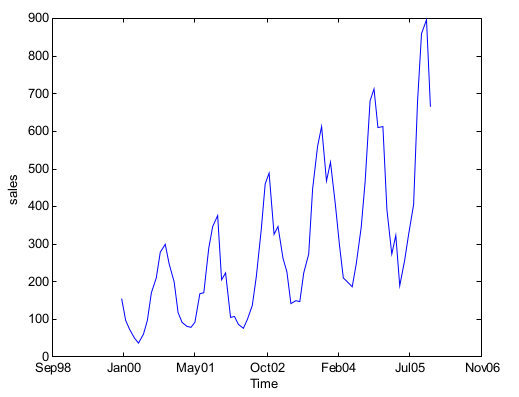
\includegraphics[scale=0.7]{graf2.png}\\   
\textbf{Σχήμα 2.1: Γράφημα χρονοσειράς}
\end{center} 
\linespread{1}

Για την ανάλυση των χρονοσειρών χρησιμοποιούμε τους ακόλουθους
συμβολισμούς:\\
\\
$Y_t$= Πραγματική τιμή της χρονοσειρά\\
$T_t$= Τάση\\
$S_t$= Εποχικότητα\\
$C_t$= Κυκλικότητα\\
$I_t$= Τυχαίες κινήσεις\\  \\
όπου $t = 1,2,3,\ldots,n$.\\


Η εξέταση των στοιχείων αυτών γίνεται σύμφωνα με κάποιο μαθηματικό
υπόδειγμα που φανερώνει τον τρόπο με τον οποίο οι παρατηρήσεις της χρονοσειράς
προσδιορίζονται από τις συνιστώσες της χρονοσειράς. Τα χρησιμοποιούμενα υποδείγματα είναι το προσθετικό μοντέλο (additive model) και το πολλαπλασιαστικό
μοντέλο (multiplicative model).

Στο προσθετικό μοντέλο οι πραγματικές τιμές της χρονοσειράς για κάθε περίοδο
θεωρούνται ως το άθροισμα των τεσσάρων συνιστωσών και δημιουργούνται με τον
ακόλουθο τρόπο:\\
$$ Y_t=T_t+S_t+C_t+I_t $$
Από την παραπάνω σχέση είναι φανερό ότι όλες οι συνιστώσες είναι εκφρασμένες
στην ίδια μονάδα μέτρησης με εκείνη των παρατηρήσεων της χρονοσειράς.

Αντίθετα στο πολλαπλασιαστικό μοντέλο οι πραγματικές τιμές της χρονοσειράς
προσδιορίζονται από το γινόμενο των τεσσάρων συνιστωσών, δηλαδή ως ακολούθως:\\
$$ Y_t=T_t \cdot S_t \cdot C_t \cdot I_t $$
Στο μοντέλο αυτό μόνο η τάση είναι εκφρασμένη στην ίδια μονάδα μέτρησης με
εκείνη της χρονοσειράς $Y_t$ ενώ τα στοιχεία $C_t$ , $S_t$ και $Ι_t$ είναι δείκτες ανεξάρτητοι
από μονάδες μέτρησης.

Από τα δύο παραπάνω μοντέλα το προσθετικό μοντέλο χρησιμοποιείται λιγότερο
συχνά στην πράξη, επειδή είναι δύσκολο στην ανάλυση του για υπολογιστικούς
κυρίως λόγους. Επίσης βασίζεται στην υπόθεση ότι οι συνιστώσες της χρονοσειράς
είναι ανεξάρτητες μεταξύ τους, που σημαίνει για παράδειγμα, ότι η τάση δεν
επηρεάζει την εποχικότητα στον υπολογισμό των τιμών της χρονοσειράς. Η
παραδοχή αυτή μπορεί να είναι σωστή κυρίως για φυσικά φαινόμενα, αλλά σπάνια
ισχύει σε επιχειρησιακές και οικονομικές εφαρμογές, στις οποίες συνήθως η τάση
επηρεάζει μεταξύ των άλλων και τις εποχικές διακυμάνσεις. Στη συνέχεια της
διπλωματικής θα χρησιμοποιήσουμε το πολλαπλασιαστικό μοντέλο, δεδομένου ότι
για τους παραπάνω πρακτικούς και θεωρητικούς λόγους το μοντέλο αυτό πλεονεκτεί
του προσθετικού για την ανάλυση των οικονομικών χρονοσειρών.

Η διάσπαση χρονοσειρών σε
αντίθεση με τις μεθόδους εξομάλυνσης, οι οποίες εφαρμόζονται κυρίως για τη
διαμόρφωση βραχυχρόνιων προβλέψεων καθώς και για χρονοσειρές με σχετικά
μικρό αριθμό παρατηρήσεων, προϋποθέτει μεγαλύτερο
αριθμό παρατηρήσεων και μπορεί να παράγει ακόμα και μακροπρόθεσμες
προβλέψεις. Η διάσπαση χρονοσειρών είναι περισσότερο χρονοβόρα σε σχέση με τις
προηγούμενες μεθόδους εξομάλυνσης, ωστόσο μας παρέχει τη δυνατότητα να
μελετήσουμε πιο διεξοδικά τον τρόπο δημιουργίας των παρατηρήσεων μιας
χρονοσειράς.

Η ανάλυση των χρονοσειρών με τη μέθοδο αυτή στηρίζεται στη διάσπαση των
παρατηρήσεων τους σε τέσσερα συνθετικά στοιχεία, δηλαδή στην \textit{τάση}, στην
\textit{εποχικότητα}, στην \textit{κυκλικότητα} και στη \textit{μη-κανονικότητα}. Σκόπος της διάσπασης των
χρονοσειρών είναι η απομόνωση των τεσσάρων παραπάνω συνθετικών στοιχείων,
ώστε να προσδιορίσουμε το βαθμό που επηρεάζει κάθε ένα στοιχείο ξεχωριστά τον
τρόπο δημιουργίας των παρατηρήσεων των χρονοσειρών. Όταν αυτό επιτευχθεί
μπορούμε να χρησιμοποιήσουμε τα αποτελέσματα της ανάλυσης για τη διαμόρφωση
προβλέψεων.\\\\
Η διαδικασία της διάσπασης (decomposistion) της χρονοσειράς απεικονίζεται
σχηματικά με το ακόλουθο διάγραμμα ροής για το πολλαπλασιαστικό μοντέλο.\\

\begin{center}
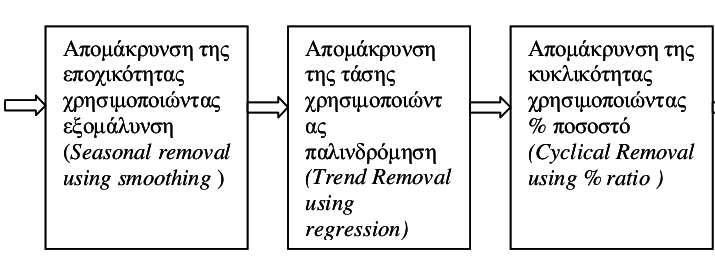
\includegraphics[scale=0.5]{graf19.png}\\   
\end{center} 
%%%%%%%%%%%%%%%%%%%%%%%%%%%%%%%%%%%%%%%%%
\subsection{ΑΝΑΛΥΣΗ ΕΠΟΧΙΚΟΤΗΤΑΣ }
%%%%%%%%%%%%%%%%%%%%%%%%%%%%%%%%%%%%%%%%%
Στην ενότητα αυτή θα παρουσιάσουμε τον τρόπο με τον οποίο μπορούμε να απαλλάξουμε τις παρατηρήσεις τις χρονοσειράς από την επίδραση της εποχικότητας. Συγκεκριμένα για τον εντοπισμό και τη μέτρηση της εποχικότητας προβαίνουμε στον υπολογισμό εποχικών δεικτών.
Εν συνεχεία, διαιρώντας τις πραγματικές τιμές της χρονοσειράς με τους
αντίστοιχους εποχικούς δείκτες τις απαλλάσσουμε από το στοιχείο της
εποχικότητας, ώστε να μπορέσουμε να διαμορφώσουμε πιο αξιόπιστες
προβλέψεις. Ακολουθεί ανάλυση της ανωτέρω διαδικασίας.\\

Για να μπορέσουμε να υπολογίσουμε τους εποχικούς δείκτες θα πρέπει
πρώτα να υπολογίσουμε τον κατάλληλο απλό κινητό μέσο. Ο κινητός μέσος
θα πρέπει να περιλαμβάνει τον ίδιο αριθμό περιόδων με αυτόν που υπάρχει
στην εποχικότητα που θέλουμε να αναγνωρίσουμε. Με άλλα λόγια, αν τα
δεδομένα της χρονοσειράς μας είναι εκφρασμένα σε τριμηνιαία βάση και
υποψιαζόμαστε ότι εμφανίζουν κάποια εποχικότητα, τότε θα πρέπει να
υπολογίσουμε τον απλό κινητό μέσο τεσσάρων περιόδων. Στην περίπτωση
που ο αριθμός των περιόδων του έτους είναι άρτιος, για παράδειγμα 4 για
τριμηνιαίες παρατηρήσεις, 6 για διμηνιαίες παρατηρήσεις και 12 για μηνιαίες παρατηρήσεις, τότε θα πρέπει να υπολογίσουμε τον κεντρικό κινητό μέσο. Αυτό συμβαίνει γιατί υπολογίζοντας μόνο τον απλό κινητό μέσο δεν υπάρχει χρονική αντιστοιχία μεταξύ των τιμών του κινητού μέσου και των τιμών της χρονοσειράς. Το πρόβλημα αυτό αντιμετωπίζεται υπολογίζοντας τον κεντρικό κινητό μέσο που δεν είναι τίποτε άλλο παρά ο μέσος δύο διαδοχικών τιμών του απλού κινητού μέσου. Σε περίπτωση που ο αριθμός των περιόδων του
έτους είναι περιττός, για παράδειγμα 3 για τετραμηνιαίες παρατηρήσεις, τότε δεν υφίσταται πρόβλημα χρονικής αντιστοιχίας μεταξύ των τιμών του κινητού μέσου και των τιμών της χρονοσειράς και ο υπολογισμός του απλού κινητού μέσου μας αρκεί για τον υπολογισμό των εποχικών δεικτών.\\

Έχοντας υπολογίσει τον απλό ή τον κεντρικό κινητό μέσο, ανάλογα με τον
αριθμό περιόδων του έτους, είμαστε σε θέση να υπολογίσουμε τους
εποχικούς δείκτες. Οι εποχικοί δείκτες προκύπτουν από τη διαίρεση των
τιμών της χρονοσειράς με τον κινητό μέσο (απλό ή κεντρικό). Έτσι,
%Η εποχικότητα είναι ένα από τα τέσσερα συνθετικά στοιχεία των χρονοσειρών
%που πρέπει να μελετηθεί, όταν στις παρατηρήσεις τους εμφανίζεται κάποιο εποχικό
%πρότυπο. Η εποχικότητα μετριέται με τους δείκτες εποχικότητας (seasonal indices),
%σκοπός των οποίων είναι η ανίχνευση του τρόπου συμπεριφοράς των παρατηρήσεων
%της χρονοσειράς που προκαλείται από αυτό το εποχικό φαινόμενο. Ο προσδιορισμός
%των δεικτών αυτών συμβάλλει στην απαλλαγή των τιμών της χρονοσειράς από το
%στοιχείο της εποχικότητας, ώστε να δημιουργηθούν πιο αξιόπιστες βραχυπρόθεσμες
%και μεσοπρόθεσμες προβλέψεις.
%Οι δείκτες εποχικότητας προσδιορίζονται με την εφαρμογή της μεθόδου του
%κεντρικού κινητού μέσου (centered moving average) στις παρατηρήσεις της
%χρονοσειράς. Με τη μέθοδο αυτή προσπαθούμε να απομονώσουμε την εποχικότητα
%από τα άλλα τρία συνθετικά στοιχεία της χρονοσειράς, δηλαδή από την τάση, την
%κυκλικότητα και τη μη-κανονικότητα.
στην περίπτωση του πολλαπλασιαστικού μοντέλου ο δείκτης εποχικότητας $S_t$ της
περιόδου $t$, για $t = 1, 2,\ldots, n$, καθορίζεται από την ακόλουθη σχέση:
$$ S_t=\frac{Y_t}{CA_t}=\frac{T_t\cdot S_t \cdot C_t \cdot I_t}{T_t \cdot C_t \cdot I_t} $$
όπου $CA_t$ είναι η εξομαλυνθείσα τιμή της χρονοσειράς που προέρχεται από τη μέθοδο
του κεντρικού κινητού μέσου που χρησιμοποιήθηκε. Έτσι η εποχικότητα
προσδιορίζεται από το λόγο των πραγματικών τιμών $Y_t$ της χρονοσειράς προς τις
εξομαλυνθείσες τιμές της $CA_t$ , θεωρώντας ότι οι τιμές $CA_t$ εκφράζουν ικανοποιητικά
την ταυτόχρονη συμπεριφορά της τάσης, της κυκλικότητας και της μη-
κανονικότητας.Επειδή το πολλαπλασιαστικό υπόδειγμα προϋποθέτει ότι το άθροισμα των εποχικών δεικτών είναι ίσο με τον αριθμό των περιόδων, αν κάτι τέτοιο δεν ισχύει τότε θα πρέπει να αναπροσαρμόσουμε τους εποχικούς δείκτες. Το άθροισμα των προσαρμοσμένων εποχικών δεικτών είναι ίσο με τον αριθμό των περιόδων. Η
προσαρμογή γίνεται αν πολλαπλασιάσουμε τον κάθε εποχικό δείκτη με το κλάσμα : αριθμός περιόδων / άθροισμα εποχικών δεικτών.\\
%Το πολλαπλασιαστικό μοντέλο προϋποθέτει να είναι το άθροισμα των εποχικών
%δεικτών ίσο με τον αριθμό των περιόδων εντός του έτους. Εάν αυτό δεν ισχύει θα
%πρέπει να γίνει κατάλληλη αναπροσαρμογή τους ώστε το άθροισμα των τιμών των
%δεικτών να ισούται με τον αριθμό των περιόδων. Οι δείκτες που προκύπτουν στην
%περίπτωση αυτή ονομάζονται προσαρμοσμένοι εποχικοί δείκτες (adjusted seasonal
%indices).

Αφού υπολογίσουμε τους προσαρμοσμένους εποχικούς δείκτες, μπορούμε στη
συνέχεια να απαλείψουμε την εποχικότητα, διαιρώντας κάθε τιμή $Y t$ της χρονοσειράς
με τον προσαρμοσμένο δείκτη $SA_i$ της αντίστοιχης περιόδου, δηλαδή ως εξής:\\
$$ SAY_t=\frac{Y_t}{SA_i} $$
όπου $SAY_t$ είναι οι απαλλαγμένες από εποχικότητα (seasonally adjusted) τιμές της
χρονοσειράς της περιόδου $t$. Οι τιμές αυτές περιέχουν την τάση, την κυκλικότητα και
τη μη-κανονικότητα.
%%%%%%%%%%%%%%%%%%%%%%%%%%%%%%%%%%%%%%%%%%%%%%%%
\subsection{ΑΝΑΛΥΣΗ ΜΑΚΡΟΧΡΟΝΙΑΣ ΤΑΣΗΣ}
%%%%%%%%%%%%%%%%%%%%%%%%%%%%%%%%%%%%%%%%%%%%%%%%
Στην ενότητα αυτή θα χρησιμοποιήσουμε τις απαλλαγμένες από εποχικότητα
τιμές της χρονοσειράς για να μελετήσουμε το άλλο συνθετικό της στοιχείο που είναι
η τάση. Η τάση φανερώνει τη μακροχρόνια εξέλιξη των τιμών της χρονοσειράς
(ανοδική ή πτωτική), η οποία οφείλεται σε δημογραφικούς, τεχνολογικούς,
οικονομικούς και άλλους παράγοντες. Για τον προσδιορισμό της θα υποθέσουμε ότι
αυτή μπορεί να εκφραστεί ικανοποιητικά από ένα γραμμικό υπόδειγμα στο οποίο ως
ανεξάρτητη μεταβλητή θα είναι ο χρόνος. Έστω ότι η τάση δίνεται από το ακόλουθο
γραμμικό υπόδειγμα:\\
\begin{equation}
\label{palin}
Y_t=\alpha +\beta \cdot t + \varepsilon_t
\end{equation}
όπου $Y_t$ είναι οι παρατηρήσεις της χρονοσειράς, $t$ η ανεξάρτητη μεταβλητή του
χρόνου που λαμβάνει τιμές $1, 2,\ldots,n\:$ και $\varepsilon$ το τυχαίο σφάλμα. Οι εκτιμήσεις των
συντελεστών της παραπάνω σχέσης προσδιορίζονται με τη μέθοδο των ελαχίστων
τετραγώνων OLS ως εξής:\\
$$ \beta= \frac{n\sum_{t=1}^n t \cdot Y_t -\left(\sum_{t=1}^n t \right) \left( \sum_{t=1}^n Y_t \right)}{n \sum_{t=1}^n t^2 -\left( \sum_{t=1}^n t \right)^2} $$
και\\
$$ \alpha=\frac{1}{n} \sum_{t=1}^n Y_t -\beta \frac{1}{n} \sum_{t=1}^n t $$
Η τιμή του $\alpha $ είναι η σταθερά της γραμμικής τάσης, δηλαδή η τιμή της τάσης όταν
$t=0$. Αντίθετα, η τιμή του $\beta $ είναι η κλίση της γραμμικής τάσης και δηλώνει το πόσο
θα μεταβληθεί η τιμή της χρονοσειράς, όταν ο χρόνος $t$ μεταβληθεί κατά μια μονάδα.
Έτσι όταν η τιμή του $\beta $ είναι θετική, η μακροχρόνια τάση είναι ανοδική, ενώ όταν η
τιμή του είναι αρνητική, η μακροχρόνια τάση είναι πτωτική.

Η τάση είναι το μόνο συνθετικό στοιχείο της χρονοσειράς που μπορούμε να
καθορίσουμε, ανεξάρτητα από την ύπαρξη ή όχι εποχικότητας στις τιμές της
χρονοσειράς. Όταν δεν υπάρχει εποχικότητα οι συντελεστές της σχέσης $\left(\ref{palin}\right)$
προσδιορίζονται χρησιμοποιώντας ως εξαρτημένη μεταβλητή τις πραγματικές τιμές
$Y_t$ της χρονοσειράς. Αντίθετα, όταν υπάρχει εποχικότητα, η $Y_t$ είναι η $SY_t$ , δηλαδή
οι απαλλαγμένες από εποχικότητα τιμές της χρονοσειράς. Στην περίπτωση αυτή, οι
παρατηρήσεις της χρονοσειράς περιέχουν την τάση, την κυκλικότητα και τη μη-
κανονικότητα, δηλαδή οι τιμές $SAY_t$ προσδιορίζονται ως:\\
$$ SAY_t=T_tC_tI_t $$
Οι τιμές $SAY_t$ χρησιμοποιούνται στη συνέχεια για την εκτίμηση της γραμμικής
τάσης:\\
$$ T_t=\alpha + \beta t $$
για όλες τις τιμές του $t$, δηλαδή για $t = 1, 2,\ldots, n$.
%%%%%%%%%%%%%%%%%%%%%%%%%%%%%%%%%%%%%%%%%%%%%%%%%%%%%%%%
\subsection{ΑΝΑΛΥΣΗ ΚΥΚΛΙΚΟΤΗΤΑΣ ΚΑΙ ΜΗ ΚΑΝΟΝΙΚΟΤΗΤΑΣ}
%%%%%%%%%%%%%%%%%%%%%%%%%%%%%%%%%%%%%%%%%%%%%%%%%%%%%%%%
Για να μελετήσουμε τα στοιχεία της κυκλικότητας και της μη-κανονικότητας της
χρονοσειράς πρέπει πρώτα να απομονώσουμε την κυκλικότητα και τη μη-
κανονικότητα από τα άλλα δύο συνθετικά στοιχεία της χρονοσειράς. Η απομόνωση
αυτή γίνεται με την απαλλαγή της τάσης από τις ήδη απαλλαγμένες από εποχικότητα
τιμές της χρονοσειράς. Συνεπώς\\
$$ TAY_t=\frac{SAY_t}{T_t}=C_tI_t $$
όπου $TAΥ_t$ είναι οι τιμές της χρονοσειράς οι απαλλαγμένες από εποχικότητα και από
την τάση (trend adjusted), δηλαδή οι τιμές αυτές περιέχουν μόνο την κυκλικότητα και
τη μη-κανονικότητα.

Η κυκλικότητα και η μη-κανονικότητα εκφράζονται ως ποσοστό της τάσης και
είναι δείκτες ανεξάρτητοι από τη μονάδα μέτρησης των παρατηρήσεων της
χρονοσειράς, όπως οι εποχικοί. Αν ο λόγος $SAY_t/ T_t$ είναι ίσος με τη μονάδα για
όλες τις παρατηρήσεις της χρονοσειράς, τότε τα στοιχεία της κυκλικότητας και της
μη-κανονικότητας δεν εμφανίζονται στις παρατηρήσεις της χρονοσειράς.
Διαγραμματικά αυτό σημαίνει ότι όλες οι απαλλαγμένες από εποχικότητα τιμές της
χρονοσειράς βρίσκονται στην εκτιμηθείσα γραμμή της τάσης. Αντίθετα, αν ο λόγος
$SAY_t/ T_t$ δεν ισούται με τη μονάδα, που είναι και η πλέον συνηθισμένη περίπτωση,
τότε στις παρατηρήσεις της χρονοσειράς υπάρχει κυκλικότητα και μη-κανονικότητα
που προσδιορίζεται από το λόγο αυτό.

Εάν ενδιαφερόμαστε να απομονώσουμε την κυκλικότητα από τη μη-
κανονικότητα τότε εφαρμόζουμε τη μέθοδο του σταθμικού κεντρικού κινητού μέσου
(weighted centered moving average) στα απαλλαγμένα από εποχικότητα και τάση
δεδομένα της χρονοσειράς. Ο σταθμικός κεντρικός κινητός μέσος δίνει μεγαλύτερη
βαρύτητα στην κεντρική παρατήρηση και μικρότερη όσο απομακρυνόμαστε χρονικά
από αυτή. Οι συντελεστές βαρύτητας ορίζονται από τον ερευνητή, ανάλογα με το
είδος των δεδομένων (μηνιαία, διμηνιαία κ.τ.λ.), ενώ το άθροισμα τους πρέπει να
είναι ίσο με τη μονάδα.

Για παράδειγμα ένας σταθμικός κεντρικός κινητός μέσος $WA_t$ για τριμηνιαία
δεδομένα θα μπορούσε να ήταν:\\
$$ WA_t=\frac{Y_{t-1}+2Y_t+Y_{t+1}}{4} $$
όπου $t = 1, 2,\ldots,n-1$ και $Y_t$ είναι τα απαλλαγμένα από εποχικότητα και τάση
δεδομένα της χρονοσειράς. Από την παραπάνω σχέση είναι φανερό ότι το άθροισμα
των συντελεστών βαρύτητας ισούται με τη μονάδα και ότι ο συντελεστής του
κεντρικού τριμήνου έχει διπλάσια βαρύτητα από τους συντελεστές του προηγούμενου
και του επόμενου τριμήνου.

Στην πραγματικότητα, με τη μέθοδο του σταθμικού κεντρικού κινητού μέσου
εξομαλύνουμε τα απαλλαγμένα από εποχικότητα και τάση δεδομένα της
χρονοσειράς. Οι εξομαλυνθείσες τιμές που προκύπτουν είναι δείκτες, οι τιμές των
οποίων είναι μικρότερες, ίσες ή μεγαλύτερες της μονάδας και φανερώνουν την
ποσοστιαία μεταβολή της τιμής της χρονοσειράς που οφείλεται στην κυκλικότητα για
κάθε χρονική περίοδο. Έτσι αν η τιμή του $WA_t$ είναι ίση με 1,36 , αυτό σημαίνει ότι
για τη συγκεκριμένη περίοδο υπάρχει αύξηση κατά 36\% στην τιμή της χρονοσειράς,
που οφείλεται στην κυκλικότητα. Εάν πάλι η τιμή του WAt είναι 0,88 τότε υπάρχει
μείωση κατά 12\% στην τιμή της χρονοσειράς που προέρχεται από το συνθετικό
στοιχείο της κυκλικότητας.

Τέλος μπορούμε να απομονώσουμε τη μη-κανονικότητα εάν απομακρύνουμε την
κυκλικότητα από τα απαλλαγμένα από εποχικότητα και τάση δεδομένα της
χρονοσειράς. Αυτό επιτυγχάνεται με τον ακόλουθο τρόπο:\\
$$ CAY_t=\frac{TAY_t}{WA_t}=I_t $$
όπου $CAY_t$ είναι οι τιμές της χρονοσειράς οι απαλλαγμένες και από την κυκλικότητα
(cyclical adjusted). Έτσι, οι τιμές αυτές περιέχουν μόνο το στοιχείο της μη
κανονικότητας.
%%%%%%%%%%%%%%%%%%%%%%%%%%%%%%%%%%%%%%%%%%
\subsection{ΔΙΑΜΟΡΦΩΣΗ ΠΡΟΒΛΕΨΕΩΝ}
%%%%%%%%%%%%%%%%%%%%%%%%%%%%%%%%%%%%%%%%%%
Η διαμόρφωση των προβλέψεων εξαρτάται σε μεγάλο βαθμό από τη διαδικασία
αναγνώρισης των συνθετικών στοιχείων ή συνιστωσών της χρονοσειράς. Όσο
καλύτερη είναι η αναγνώριση των στοιχείων αυτών, τόσο καλύτερη αναμένεται να
είναι και η πρόβλεψη των τιμών της χρονοσειράς. Έτσι, κάθε ένα συνθετικό στοιχείο
χρησιμοποιείται ξεχωριστά για τον προσδιορισμό των μελλοντικών τιμών της
χρονοσειράς. Ειδικότερα, η πρόβλεψη $\widehat{Y}_{t+h}$ της $h$ μελλοντικής περιόδου
προσδιορίζεται με βάση το πολλαπλασιαστικό μοντέλο ως εξής:\\
$$ \widehat{Y}_{t+h}=T_{t+h}S_{t+h}C_{t+h}I_{t+h} $$

Η τιμή του $I_{t+h}$ , δηλαδή η συμβολή της μη κανονικότητας για την h μελλοντική
περίοδο, δεν μπορεί να καθοριστεί, αφού εξαρτάται από τυχαίους και απρόσμενους
παράγοντες και κατά συνέπεια δεν μπορεί να προσδιοριστεί. Για το λόγο αυτό, η μη-
κανονικότητα δεν περιλαμβάνεται στη διαμόρφωση των προβλέψεων και έτσι η τιμή
του $I_{t+h}$ τίθεται ίση με τη μονάδα, δηλαδή:\\
$$ I_{t+h}=1 $$

Όσον αφορά την κυκλικότητα, αν οι κυκλικές διακυμάνσεις είναι μεγάλες τότε
συμπεριλαμβάνονται στην πρόβλεψη ενώ αν οι κυκλικές διακυμάνσεις είναι μικρές,
δηλαδή οι τιμές $WA_t$ είναι κοντά στη μονάδα, τότε το $C_{t+h}$ δεν περιλαμβάνεται στη
διαμόρφωση των προβλέψεων και θεωρούμε ότι η τιμή του είναι ίση με τη μονάδα,
δηλαδή:\\
$$ C_{t+h}=1 $$
Για την τιμή του $S_{t+h}$ , δηλαδή για την τιμή του δείκτη εποχικότητας της h
μελλοντικής περιόδου, χρησιμοποιούμε την τιμή του προσαρμοσμένου δείκτη
εποχικότητας SA της περιόδου εντός του έτους στην οποία αναφέρεται η h
μελλοντική περίοδος, δηλαδή:\\
$$ S_{t+h}=SA_i $$
για $i = 1, 2,\ldots,L$ , όπου L είναι η περιοδικότητα της εποχικότητας.

Τέλος, η τιμή του $T_{t+h}$ , δηλαδή η τιμή της τάσης της h μελλοντικής περιόδου,
προκύπτει από τη σχέση ως εξής:\\
$$ T_{t+h}=\alpha+\beta \left(t+h\right) $$
όπου $\alpha$ και $\beta$ οι συντελεστές της γραμμικής τάσης.

Επομένως οι προβλέψεις των τιμών της χρονοσειράς για την h μελλοντική
περίοδο δημιουργούνται από την ακόλουθη σχέση:\\
$$ \widehat{Y}_{t+h}=\left[\alpha+\beta\left(t+h\right)\right]SA_i  $$
όπου έχουμε θεωρήσει $I_{t+h} = 1$ και $C_{t+h} = 1$, δηλαδή λαμβάνουμε υπ’όψιν μόνο την
τάση και την εποχικότητα.
%%%%%%%%%%%%%%% File ends here %%%%%%%%%%%%%%%%%%%%%%%%%%%%%%%%
\endinput
%%% Local Variables: 
%%% mode: latex
%%% TeX-master: "ptyxiakn"
%%% End: 
